\documentclass[9pt]{article}
\usepackage[utf8]{inputenc}
\usepackage{amsmath,amsthm,amsfonts,amssymb,amscd}
\usepackage{multirow,booktabs}
\usepackage{enumitem}
\usepackage{fancyhdr}
\usepackage{mathrsfs}
\usepackage{wrapfig}
\usepackage{setspace}
\usepackage{calc}
\usepackage{multicol}
\usepackage{cancel}
\usepackage[retainorgcmds]{IEEEtrantools}
\usepackage{framed}
\usepackage[most]{tcolorbox}
\usepackage{tikz}
\usepackage{geometry}
\geometry{
	a4paper,
	total={170mm,257mm},
	left=20mm,
	top=20mm,
}
\title{Gravity}
\author{Aaron G.K.}

\begin{document}
	\maketitle
	\begin{center}
	\section*{Newton's Law of Universal Gravitation}	
	\end{center}
	\subsection*{Gravity}
	Before Newton's discovery, people used to think that the laws that govern interactions on Earth were different to the ones that govern the "heavens" - the space outside the Earth. With Newton's discovery, he was able to explain and properly quantify that the force that govern the falling of an apple is indeed the same one that governs the rotation of the moon around the Earth. With this in mind, he came with what we know today as \textit{Newton's Law of Universal Gravitation.} In that law, he states that
	\begin{quote}
		The force of gravity between any two point objects of mass $m_1$ and $m_2$ is attractive and of magnitude
		$$F=\dfrac{Gm_1m_2}{r^2}\text{,           where G = }6.672\times10^{-11}\text{Nm}^2/\text{kg}^2	$$
		and is acted along the line connecting the masses.
	\end{quote}
	In our equation above, \textit{r} is the distance between our objects and G is a constant called the gravitational constant. It was first calculated by Henry Cavendish(yes, the same guy who discovered Hydrogen). One important proposal by Newton in his law was that all objects in the universe attract the other objects by a way of gravitational interaction. 
	\subsubsection*{Weighing the Earth}
	After Newton came forward with his law, Henry Cavendish determined the gravitational constant with a staggering accuracy having an experimental setup similar to the figure below.
	\begin{center}
		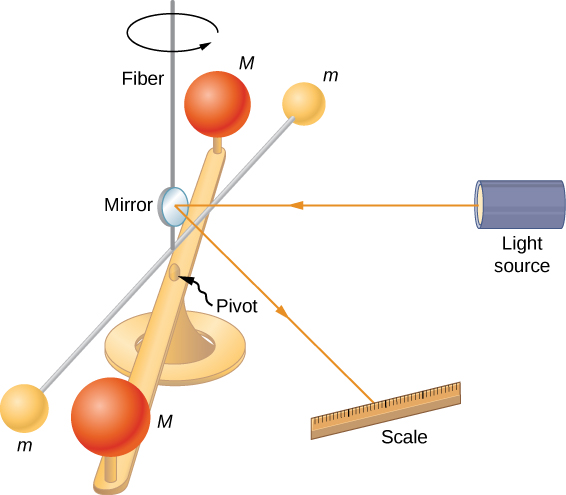
\includegraphics[scale=0.7]{weighing_the_earth.jpeg}	
	\end{center}
	Cavendish new the amount of torsional force needed to rotate the supporting wire(fiber) through some angle. Once in equilibrium, two fixed, larger masses are placed symmetrically near the smaller ones. The gravitational attraction creates a torsion (twisting) in the supporting wire that can be measured, since he already knew the amount of force needed to rotate the fiber, he measured the angle the fiber rotated through and he determined the force between the larger and smaller masses - effectively measuring the force of gravity between them.
	$$\text{F}\propto\dfrac{\text{mM}}{\text{r}^2}$$
	We know the proportional constant is G:
	$$\text{F} = G\dfrac{\text{mM}}{\text{r}^2}$$
	We can then express G in terms of the force of gravitational force, the masses \& the separation:
	$$\text{G} = \dfrac{\text{Fr}^2}{\text{mM}}$$
	With the relationship above, he was able to determine the gravitational constant. With the gravitational constant being determined, Newton's idea of gravity being a universal force of attraction was codified. Cavendish determined G, but why is the experiment he did called \textit{Weighing the Earth}? By the time he did the experiment, Earth's radius and acceleration due to gravity was already determined, so once the value of G was known, people could calculate the mass of the Earth. \\
	If an object is acted upon by gravitational interactions with different masses, we find the net force by computing the vector sum. This property of gravity is called superposition(similar to how we add up waves during interference). 
	\subsubsection*{Acceleration Due to Gravity}
	We now know that the force of gravity between two masses is given by Newton's Law of Universal Gravitation. For daily activities as humans, we don't really move away from the surface of the Earth, even for the high altitude flights, the distance from the surface the plane is at is very small compared to the radius of the Earth. Thus, we can assume r is somewhat constant for all of us folks here on Earth. With that, we can calculate the acceleration due to gravity one feels while on here. Let \textbf{m} be the mass of an object on Earth who has a mass of \textbf{M}. The force of attraction between \textbf{m} and \textbf{M} is given by:
	$$F=\dfrac{GmM}{r^2}$$
	We also know that if we propel m into the air, it comes down to the surface: it has an acceleration. Thus, the net force on it is given by:
	$$\textbf{F}=m\textbf{a}$$
	We do know that these two forces are the same, thus we equate them and we get:
	$$m\textbf{a}=\dfrac{GmM}{r^2}$$	
	$$\textbf{a}=\dfrac{GM}{r^2}$$	
	Thus, we find that the acceleration due to gravity  doesn't depend on the mass of the object, but rather depends on the mass of Earth. Recall that we never cared about the mass of projectiles while discussing their motion. This is why.
	\subsubsection*{Gravitational Potential Energy}
	Potential energy is a type of energy that is attained due to having some state in a field. You have seen multiple types of potential energies in the past; electrical potential energy, elastic potential energy, chemical potential energy, and now gravitational potential energy. Gravitational Potential Energy(GPE) is defined to be 0 at infinity(since we have no influence of the force at infinity - recall that gravitational force has an inverse square relationship with distance from the source.) Thus, if an object \textbf{m} is at a distance of \textbf{r} from a larger mass \textbf{M}, the force, $\text{F}\to0\text{ when r}\to\infty$. The potential energy possessed by m at a distance of r is the amount of work one would need to do to move \textbf{m} from the source to its position r. Thus,
	$$\text{GPE}=\text{Fr}$$
	$$\text{GPE}=\dfrac{\text{GmM}}{r^2}r$$
	$$\text{GPE}=\dfrac{\text{GmM}}{r}$$
	We represent GPE by U and from our definition above, we get a generalized form:
	$$\text{U}=-\dfrac{\text{GmM}}{r}$$
	Knowing the GPE has many important values. For one, if we want to make our satellites move out of the Earth, they have to escape the pull by Earth's gravity. To escape the potential well, we have to have do work that is at least equal to the GPE. The work we do is manifested through the kinetic energy of the satellite we intend to propel. Thus, we have the following: \\
	Gravitational Potential Energy of the Satellite-Earth System = Kinetic Energy of the Satellite \\
	If my satellite has a mass \textbf{m} and the Earth has a mass M, the following is true:
	$$\dfrac{\text{GmM}}{\text{r}^2}=\dfrac{1}{2}\text{m}v^2$$
	$$\dfrac{\text{GM}}{\text{r}^2}=\dfrac{1}{2}v^2$$
	$$v=\sqrt{2\dfrac{GM}{r}}$$
	We can also express the velocity in terms of \textit{g}.
	$$v=\sqrt{2\dfrac{GM}{r^2}r}$$
	$$v=\sqrt{2gr}$$
	The velocity above is the minimum velocity an object must move with so that it can escape the pull of the Earth. It is an important information because we can see that the mass of the object has	nothing to do with the value of the velocity.
	\subsubsection*{Orbital Velocity}
	We have seen above that satellites or objects need to travel at some threshold speed to escape the pull the Earth has on them. What about when the satellite needs to stay in orbit? What does it need to do? Well, we see, again, that the satellite would need to travel at some threshold velocity. Recall from our lesson earlier in the semester about centripetal force - the force that keeps an objects trajectory circular. Making an assumption that satellites have a circular path(which rarely is the case, but easy math),we can determine their orbital speeds. Newton told us it is gravity that makes planets rotate around the sun and we know that it is indeed gravity that makes satellites rotate around the Earth. Thus, we have: \\
	
	The centripetal force needed to keep the satellite in orbit = the force of attraction between the planet and the satellite \\ 
	
	$$\dfrac{mv^2}{r}=\dfrac{GmM}{r^2}$$
	$$v=\sqrt{\dfrac{GM}{r}}$$
	Again, the orbital velocity only depends on what's being orbitted and the distance from it, not the mass of the orbitting object.
	We can also express the velocity in terms of \textit{g}.
	$$v=\sqrt{\dfrac{GM}{r^2}r}$$
	$$v=\sqrt{gr}$$
	
	\end{document}	